\section{High Level Design}
\label{sect:high_level_design}

Included below in the following sub-sections (Section~\ref{sect:architectural_diagram}~and Section~\ref{sect:activity_diagram}) are an architectural diagram and activity diagram which describe some high-level design features of PyBank.

\subsection{System-Level Structural Diagram}
\label{sect:architectural_diagram}

The high-level components of PyBank can be listed broadly as the following:
\begin{itemize}
    \item {PyBank PyQt5 GUI}
    \item {Navigation Menu Component}
    \item {Login Component}
    \item {Sign-up Component}
    \item {Account Overview Component}
    \item {Checking Account Component}
        \begin{itemize}
            \item {Show Graphs Component}
            \item {Deposit Component}
            \item {Withdraw Component}
        \end{itemize}
    \item {Savings Account Component}
        \begin{itemize}
            \item {Show Graphs Component}
            \item {Deposit Component}
            \item {Withdraw Component}
        \end{itemize}
    \item {Credit Card Account Component}
        \begin{itemize}
            \item {Show Graphs Component}
            \item {Make A Payment Component}
            \item {Request Credit Line Increase Component}
        \end{itemize}
    \item {CSV File I/O Component}
\end{itemize}

The relationship between the PyBank PyQt5 GUI application and it's related components are further depicted in the architectural diagram shown below in Figure~\ref{fig:architectural_diagram}. This figure shows the components that are enclosed within the PyBank PyQt5 GUI as well as the CSV File I/O component which handles transaction processing for each PyBank customer. Unidirectional arrows convey an association between one component and another. For example, the Navigation Menu component is associated with six other components in the application. Bidirectional arrows convey both association and communication between two components in the application. Finally, dotted arrows are drawn to make it easier to visualize arrows that must cross the boundary of another arrow.

\begin{figure}[H]
	\begin{centering}
	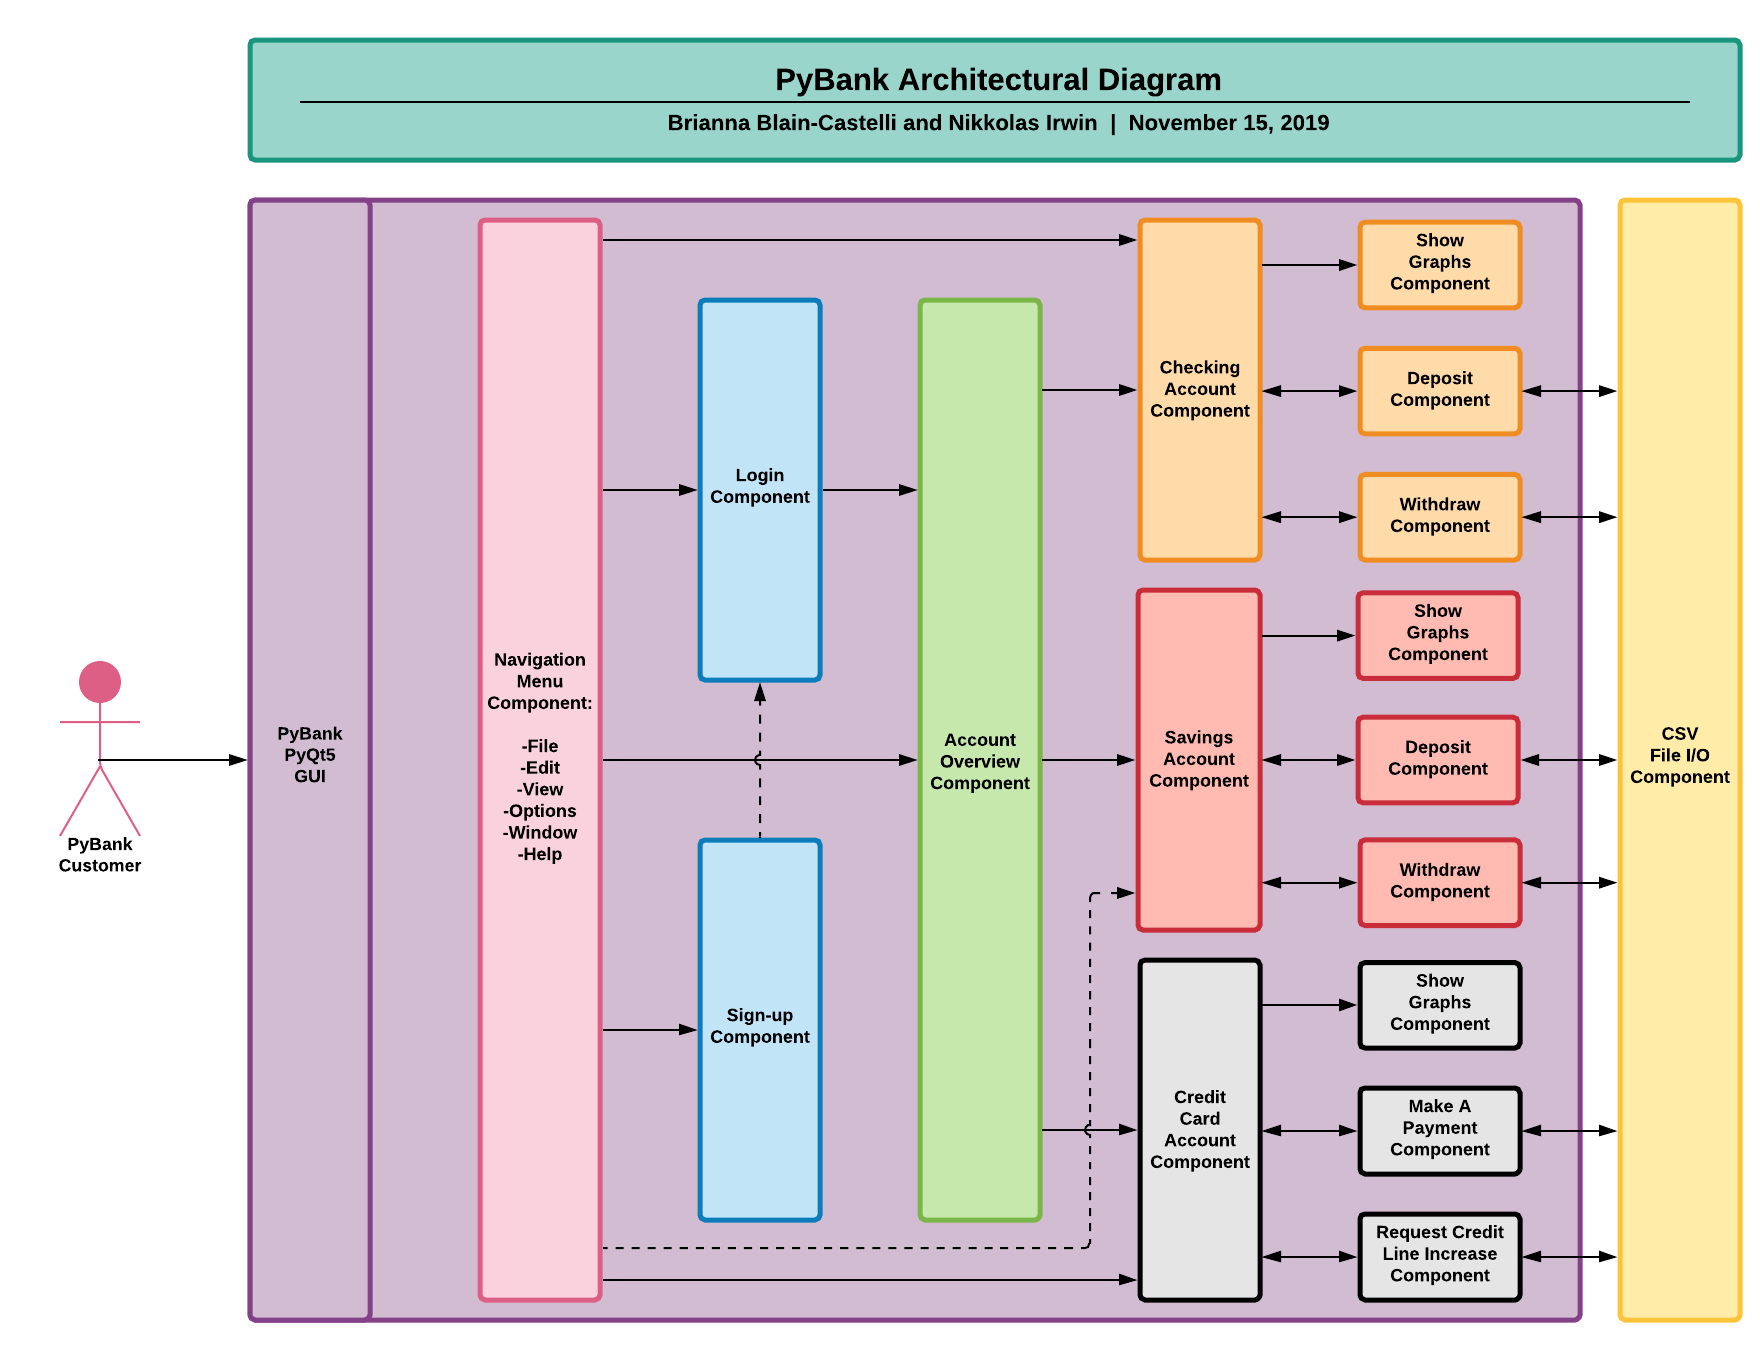
\includegraphics[width=1.00\linewidth, height=0.75\linewidth]{figures/Architectural_Diagram_PyBank.png}
	\caption{An architectural diagram describing the major software components present in PyBank.}
	\label{fig:architectural_diagram}
	\end{centering}
\end{figure}

\newpage

\subsection{System-Level Behavioral Diagram}
\label{sect:activity_diagram}

The activity diagram shown below in Figure~\ref{fig:activity_diagram} depicts the sequence of actions that a PyBank customer would take to either login to their existing account or sign-up for a new account and then log into that account. The activity begins with a PyBank customer executing the desktop client and completes once the PyBank customer has logged into their account and is presented with the \textbf{\textit{Account Overview}} window.

\begin{figure}[H]
	\begin{centering}
	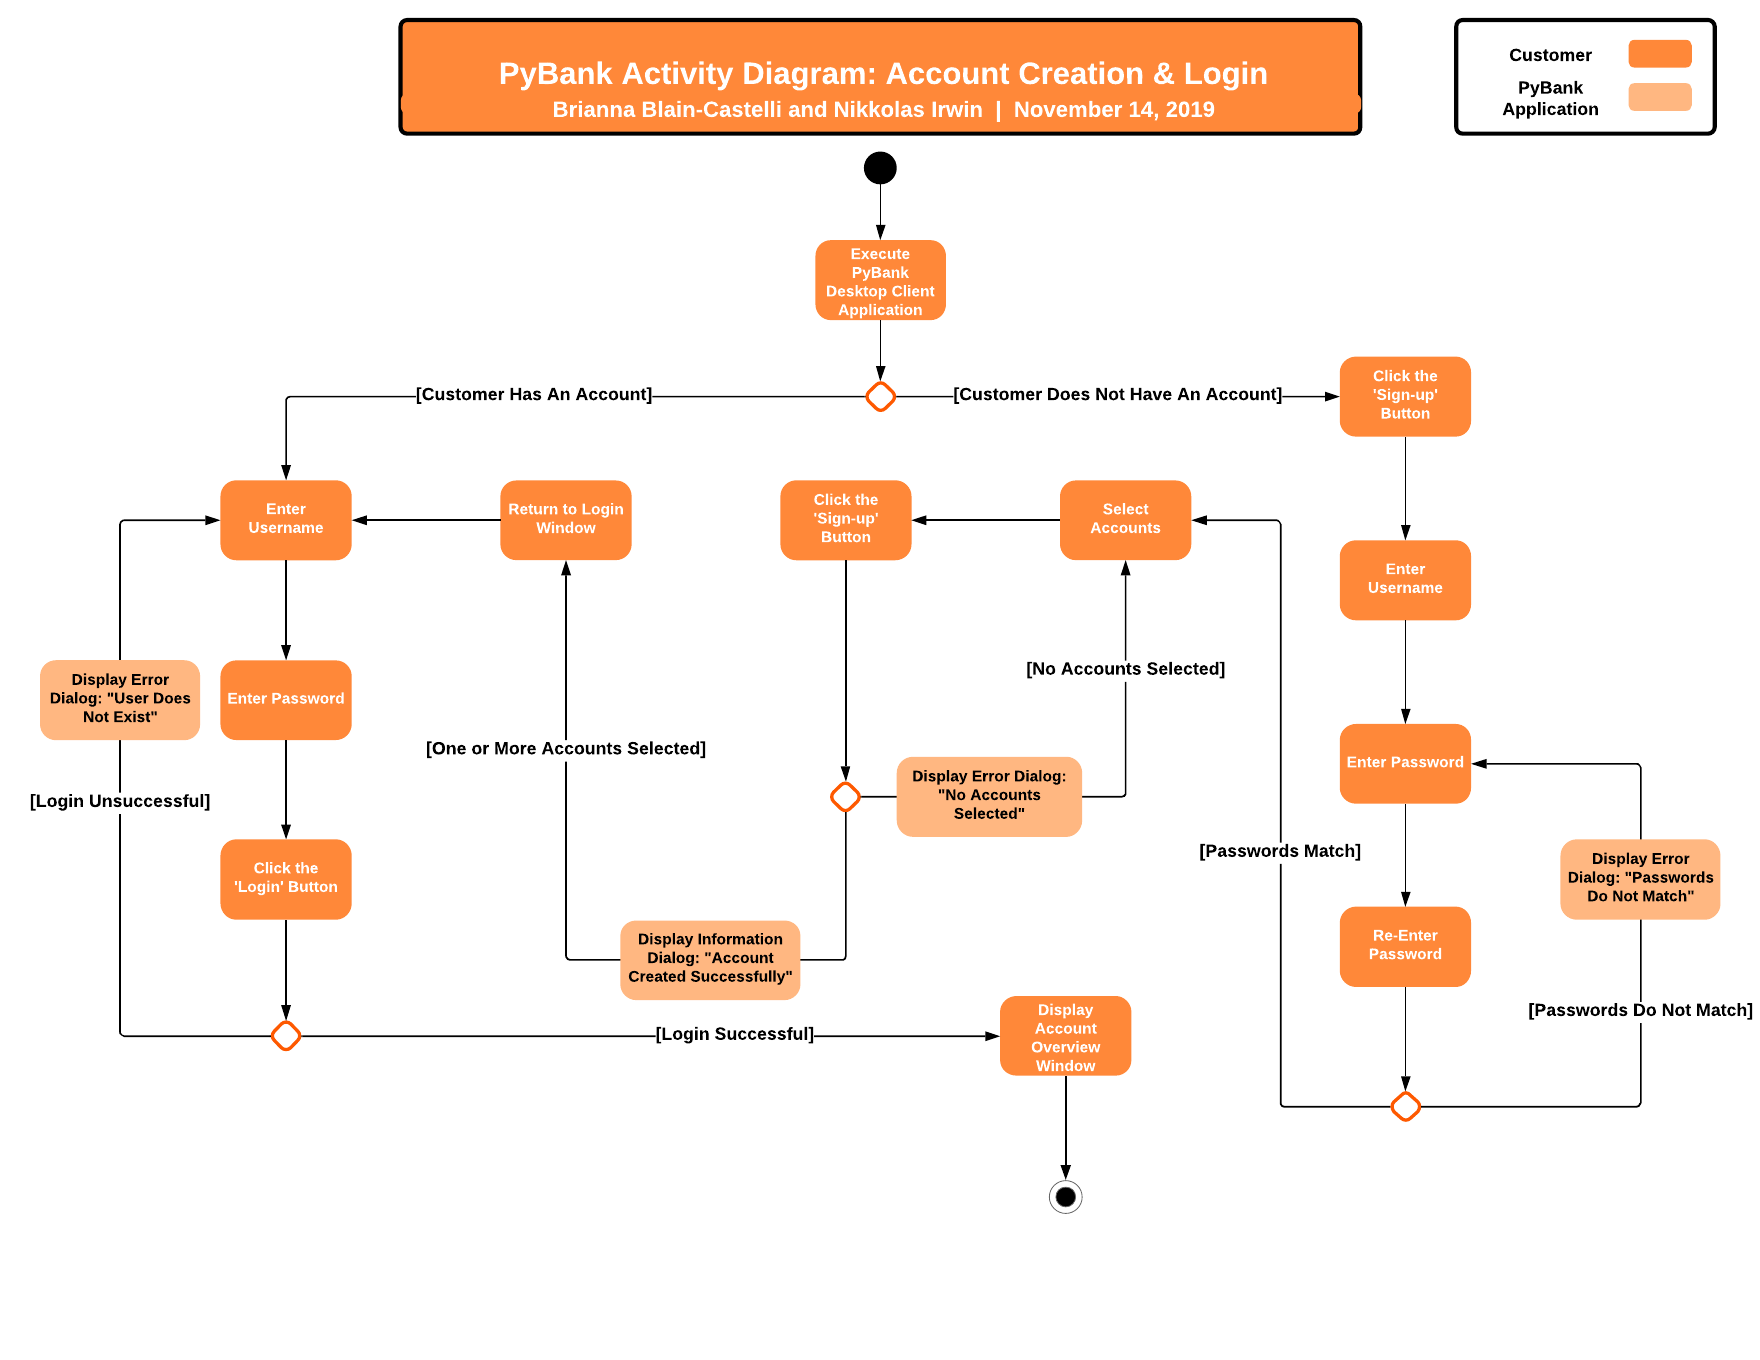
\includegraphics[width=1.00\linewidth, height=0.75\linewidth]{figures/Activity_Diagram_PyBank.png}
	\caption{An activity diagram describing the login and account creation processes in PyBank.}
	\label{fig:activity_diagram}
	\end{centering}
\end{figure}

%EOF